\documentclass[12pt]{article}

% Поддержка кириллицы
\usepackage[T2A]{fontenc}
\usepackage[utf8]{inputenc}
\usepackage[english, russian]{babel}

% Поддержка математики
\usepackage{amsmath, amssymb, amsthm}

\everymath{\displaystyle}

% Создание среды для определений
\newtheorem{definition}{Определение}

% Создание среды для доказательств
\newtheorem{theorem}{Теорема}

% Начальный отступ
\usepackage{indentfirst}

% Важная информация в рамку
\usepackage{mdframed}

% Вставка картинок правильная
\usepackage{graphicx}

%"Плавающие" картинки
\usepackage{float}

%Обтекание фигур (таблиц, картинок и прочего)
\usepackage{wrapfig}

% подписи к рисунку
\usepackage{caption}
\renewcommand{\figurename}{Рис.}
\renewcommand{\thefigure}{\arabic{figure}.}
\captionsetup[figure]{labelsep=period}

\begin{document}
	
	% Титульник
	\title{Лекции по предмету\\"Вычислительная математика"}
	\author{Тишкин Владимир Федорович}
	\date{}
	\maketitle
	\newpage
	
	\tableofcontents
	
	\section*{Лекция №1: История вычислительной математики}
\addcontentsline{toc}{section}{Лекция №1}

\subsection*{Введение}
\addcontentsline{toc}{subsection}{Введение}

Развитие численных методов и становление науки вычислительной математики связано с необходимостью решения крупных научно- технических проблем и появлением быстродействующих электронно - вычислительных машин. С 1948 года  А. А. Самарский совместно с академиком А. Н. Тихоновым разрабатывал численные методы и вел первые в СССР прямые расчеты мощности взрыва атомной, а позже — водородной бомбы, необходимые для проведения дальнейших экспериментов. В этих работах были заложены основы математического моделирования и созданы важнейшие принципы конструирования и обоснования разностных схем и параллельных вычислений. 

Успехи ядерной физики, и в первую очередь, создание атомной бомбы, атомной энергетики, искусственных спутников Земли потребовали развития и широкого применения методов математического моделирования, а вместе с этим, развития вычислительной техники и подготовки специалистов-математиков, использующих эту технику.

\subsection*{Разностная аппроксимация простейших дифференциальных операторов}
\addcontentsline{toc}{subsection}{Разностная аппроксимация}

\subsubsection*{Сетки и сеточные функции}
\addcontentsline{toc}{subsubsection}{Сетки и сеточные функции}

Для того чтобы написать разностную схему, приближенно описывающую данное дифференциальное уравнение, нужно совершить следующие два шага.

\begin{enumerate}
	\item Необходимо заменить область непрерывного изменения аргумента областью дискретного его изменения.
	\item Необходимо заменить дифференциальный оператор некоторым разностным оператором, а также сформулировать разностный аналог для краевых условий и для начальных данных.
\end{enumerate}

После осуществления такой процедуры мы приходим к алгебраической системе уравнений. Таким образом, задача о численном решении исходного (линейного) дифференциального уравнения сводится к вопросу о нахождении решения полученной алгебраической системы.

Остановимся на этих вопросах несколько подробнее.

При численном решении той или иной математической задачи мы, очевидно, нө можем воспроизвести разностное решение для всех значений аргумента, изменяющегося внутри некоторой области евклидова пространства.

Естественно поэтому выбрать в этой области некоторое конечное множество точек и приближенное решение искать только в этих точках. Такое множество точек называется сеткой. Отдельные точки называют узлами сетки.

Функция, определенная в узлах сетки, называется сеточной функцией. Таким образом, мы заменили область непрерывного изменения аргумента сеткой, т. е. областью дискретного изменения аргумента; иными словами, мы осуществили аппроксимацию пространства решений дифференциального уравнения пространством сеточных функций.

Свойства разностного решения и, в частности, его близость к точному решению зависят от выбора сетки.

\textbf{Пример 1}. Равномерная сетка на отрезке. Разобьем единичный отрезок $[0,1]$ на $N$ равных частей. Расстояние между соседними узлами $x_i-x_{i-1}=h=1 / N$ назовем шагом сетки. Точки деления $x_i=i h-$ узлы сетки. Множество всех узлов $\omega_h=\left\{x_i=\right.$ $=i h, i=1,2, \ldots, N-1\}$ и составляет сетку (рис. 1), в данном случае введенную на отрезке.

\begin{wrapfigure}{r}{0.5\textwidth}
	\centering
	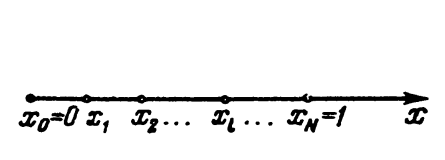
\includegraphics[width=0.5\textwidth]{img/1.png}
	\caption{}
	\label{fig:1}
\end{wrapfigure}


В это множество можно включить граничные - точки $x_0=0, \quad x_N=1$. Обозначим $\bar{\omega}_h=\left\{x_i=i h, i=0,1, \ldots\right.$ ..., $N-1, N\}$.
(рис.~\ref{fig:1}) 
На отрезке [0,1] вместо функции непрерывного аргумента $y(x)$ будем рассматривать функцию дискретного аргумента $y_h\left(x_i\right)$. Значения этой функции вычисляются в узлах сетки $x_i$, а сама функция зависит от шага сетки $h$ как от параметра.

\textbf{Пример 2}. Равномерная сетка на плоскости. Рассмотрим множество функций двух аргументов $u(x, t)$. В качестве области определения выберем прямоугольник

$$
\overline{D}=\{0 \leqslant x \leqslant 1, \quad 0 \leqslant t \leqslant T\} .
$$

\begin{wrapfigure}{r}{0.5\textwidth}
	\centering
	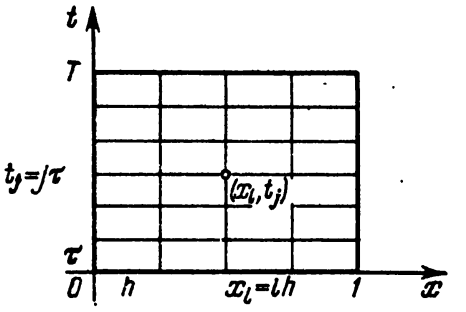
\includegraphics[width=0.5\textwidth]{img/2.png}
	\caption{}
	\label{fig:2}
\end{wrapfigure}


Разобьем отрезки $[0,1]$ оси $x$ и $[0, T]$ оси $t$ соответственно на. $N_1$ и $N_2$ частей; пусть $h=1 / N_1$, $\tau=T / N_2$. Через точки деления проведем прямые, параллельные соответствующим осям. В результате пересечения этих прямых получим узлы ( $\left.x_i, t_j\right)$, которые и образуют сетку (рис.~\ref{fig:2}) 

$$
\overline{\omega_{h \tau}}=\left\{\left(x_i, t_j\right) \in \overline{D}\right\} .
$$

Эта сетка имеет шаги $h$ и $\tau$ соответственно по направлениям $x$ и $t$. Соседними узлами сетки называются узлы, лежащие на одной и той же прямой (горизонтальной или вертикальной), расстояние между которыми равно шагу сетки ( $h$ или $\tau$ ).

\textbf{Пример 3}. Неравномерная сетка на отрезке. Рассмотрим отрезок $0 \leqslant x \leqslant 1$. Вводя произвольные точки $0<x_1<x_2<\ldots$... $\ldots<x_{N-1}<1$, разобьем его на $N$ частей. Множество узлов $$\left\{x_i : i=0, \ldots, N, \quad x_0=0, x_N=1\right\}$$ образует неравномерную сетку $\widehat{\omega}_h[0,1]$. Расстояние между соседними узлами - шаг сетки - равно $h_i=x_i-x_{i-1}$ п зависит уже от номера $i$ узла, т. е. является сеточной функцией. Шаги сетки удовлетворяют условию нормировки

$$
\sum_{i=1}^N h_i=1
$$

\textbf{Пример 4}. Сетка в двумерной области. Пусть на плоскости $x=\left(x_1, x_2\right)$ дана область $G$ сложной формы с границей $\Gamma$. Проведем прямые $x_1^{\left(i_1\right)}=i_1 h_1, i_1=0, \pm 1, \pm 2, \ldots, h_1>0 ; x_2^{\left(i_2\right)}=i_2 h_2, i_2=$ $=0, \pm 1, \pm 2, \ldots, h_2>0$. Тогда на плоскости ( $x_1, x_2$ ) получим сетку (решетку) с узлами ( $\left.i_1 h_1, i_2 h_2\right), i_1, i_2=0, \pm 1, \pm 2, \ldots$

\begin{wrapfigure}{l}{0.45\textwidth}
	\centering
	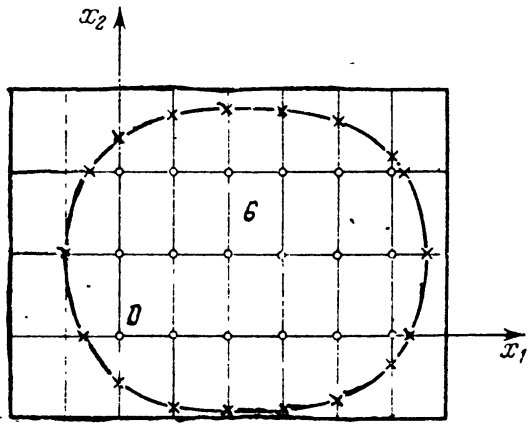
\includegraphics[width=0.45\textwidth]{img/3.png}
	\caption{}
	\label{fig:3}
\end{wrapfigure}

Эта решетка равномерна по каждому из направлений $O x_1$ и $O x_2$. Нас интересуют только те узлы, которые принадлежат области $\bar{G}=G+\Gamma$, включая границу $\Gamma$. Те узлы ( $i_1 h_1, i_2 h_2$ ), которые попали внутрь $G$, назовем внутренними, а их совокупность обозначим $\omega_h$ (рис. 3). Рассмотрим точки пересечения прямых $x_1^{\left(i_1\right)}=i_1 h_1 \quad$ и $\quad x_2^{\left(i_2\right)}=i_2 h_2$, $i_1, i_2=0, \pm 1, \pm 2, \ldots$, с границей $\Gamma$; эти точки назовем граничными узлами, а множество всех граничных узлов обозначим $\gamma_h$. На (рис.~\ref{fig:3})  знаком $\times$ обозначены граничные узлы, а значком - - внутренние узлы. Из (рис.~\ref{fig:3})  видно, что имеются граничные узлы, которые отстоят от ближайших к ним внутренних узлов на расстоянии, меньшем $h_1$ или $h_2$. Таким образом, хотя сетка на плоскости и равномерна по $x_1$ и $x_2$, но сетка $\bar{\omega}_h=\omega_h+\gamma_h$ для области $\bar{G}$ неравномерна вблизи границы.

Итак, область $\bar{G}$ изменения аргумента $x$ мы заменяем сеткой $\bar{\omega}_h$, т. е. конечным множеством точек $x_i$, принадлежащих $\bar{G}$. Вместо функций $u(x)$ непрерывного аргумента $x \in \bar{G}$ будем рассматривать сеточные функции $y\left(x_i\right)$, т. е. функции точки $x_i$, являющейся узлом сетки $\bar{\omega}_h=\left\{x_i\right\}$. Сеточную функцию $y\left(x_i\right)$ можно представить в виде вектора. Если перенумеровать все узлы в некотором порядке $x_1, x_2, \ldots, x_N$, то значения сеточной функции в этих узлах можно рассматривать как компоненты вектора

$$
Y=\left(y_1, \ldots, y_i, \ldots, y_N\right) .
$$

Если область $G$, в которой построена сетка, конечна, то размерность $N$ вектора $Y$ конечна. В случае неограниченной области $G$ сетка состоит из бесконечного числа узлов и размерность вектора $Y$ также бесконечна.

Обычно рассматриваются множества сеток $\left\{\omega_h\right\}$, зависящих от шага $h$ как от параметра. Поэтому и сеточные функции $y_h(x)$ зависят от параметра $h$ (или от числа узлов $N$ в случае равномерной сетки). Если сетка $\omega_h$ неравномерна, то под $h$ следует понимать вектор $h=\left(h_1, h_2, \ldots, h_N\right)$ с компонентами $h_1, \ldots, h_N$.

		
	\section*{Лекция №2: Анализ устойчивости численных схем}
\addcontentsline{toc}{section}{Лекция №2}

\subsection*{Введение}
\addcontentsline{toc}{subsection}{Введение}

В данной лекции мы рассмотрим понятие устойчивости численных методов. Устойчивость является ключевым аспектом при решении дифференциальных уравнений численными методами, поскольку она определяет, насколько надежным будет полученное численное решение при малых изменениях начальных условий или параметров задачи.

\subsection*{Основные понятия и определения}
\addcontentsline{toc}{subsection}{Основные понятия и определения}


Очевидно, что при аппроксимации задачи особое внимание следует обратить на запись в разностном виде начального условия для производной $\partial u / \partial t$.

Пусть дана равномерная по $x$ и $t$ сетка $\omega_{h \tau}$ с шагами $h$ и $\tau$. Если мы воспользуемся простейшей аппроксимацией
$$
u_t(x, 0)=\bar{u}_0(x),
$$

то погрешность аппроксимации будет величиной $O(\tau)$. Представим $u_t(f, 0)$ в виде
$$
u_t(x, 0)=\frac{u(x, \tau)-u(x, 0)}{\tau}=\frac{\partial u(x, 0)}{\partial t}+\frac{\tau}{2} \frac{\partial^2 u(x, 0)}{\partial t^2}+O\left(\tau^2\right) .
$$

Обратимся теперь к исходному дифференциальному уравнению и найдем
$$
\frac{\partial^2 u(x, 0)}{\partial t^2}=\frac{\partial^2 u(x, 0)}{\partial x^2}+f(x, 0)=L u_0(x)+f(x, 0), \quad L u_0=\frac{d^2 u_0}{d x^2},
$$

так как $\frac{\partial^2 u(x, 0)}{\partial x^2}=\frac{d^2 u_0(x)}{d x^2} \cdot$ Отсюда следует, что
$$
u_t(x, 0)-0,5 \tau\left(L u_0+f(x, 0)\right)=\frac{\partial u(x, 0)}{\partial t}+O\left(\tau^2\right) .
$$

Поэтому разностное начальное условие $y_t(x, 0)=\tilde{u}_0(x)$, где $\tilde{u}_0(x)=\bar{u}_0(x)+0,5 \tau\left(L u_0+f(x, 0)\right)$, аппроксимирует на решении задачи условие $\partial u(x, 0) / \partial t=\bar{u}_0(x)$ со вторым порядком по $\tau$.

Условие $u(x, 0)=u_0(x)$ и краевые условия в данном случае аппроксимируются точно. В качестве разностной аппроксимации уравнения можно взять, например, одну из схем.

Из предыдущего изложения следует, что при повышевии порядка аппроксимации краевых и начальных условий мы использовали существование и непрерывность производных, входящих в уравнение, на границе области (при $x=0$ или $t=0$ ), а также существование и ограниченность третьих производных решения.

Пример. Трехслойная разностная схема для уравнения теплопроводности. Рассмотрим первую краевую задачу
$$
\begin{aligned}
	\frac{\partial u}{\partial t} & =\frac{\partial^2 u}{\partial x^2}+f(x, t), \quad 0<x<1, \quad 0<t \leqslant t_0, \\
	u(x, 0) & =u_0(x), \quad u(0, t)=u_1(t), \quad u(1, t)=u_2(t) .
\end{aligned}
$$

Для решения уравнения теплопроводности часто применяются так называемые трехслойные схемы, использующие значения сеточной функции $y^{j-1}(x), y^j(x), y^{j+1}(x)$ на трех временных слоях $t_{j-1}, t_j, t_{j+1}$.

Например, трехслойная симметричная схема на равномерной сетке $\omega_{h г}$ с шагами $h$ и $\tau$ выглядит следующим образом:
$$
\begin{gathered}
	\frac{y^{j+1}-y^{j-1}}{2 \tau}=\Lambda\left(\sigma y^{j+1}+(1-2 \sigma) y^j+\sigma y^{j-1}\right)+\varphi^j, \\
	y_i^0=u_0\left(x_i\right), \quad y_0^j=u_1^j, \quad y_N^j=u_2^j,
\end{gathered}
$$

где $\Lambda y=y_{\overline{x} x}, \sigma$ - вещественный параметр, $\varphi^j=f\left(x_i, t_j\right)$.
Так как центральная разностная производная по $t$ аппроксимирует $\left.\frac{\partial u}{\partial t}\right|_{t=t_j}$ со вторым порядком по $\tau$, а $\Lambda u=\frac{\partial^2 u}{\partial x^2}+O\left(h^2\right)_x$ то схема аппроксимирует уравнение с $O\left(h^2+\tau^2\right)$. Heтрудно, однако, заметить, что задача не доопределена. Для применения трехслойной схемы требуется задать еще одно начальное условие, например, задать $y(x, t)$ на первом слое. Естественно потребовать, чтобы введение этого условия сохраняло аппроксимацию $O\left(\tau^2+h^2\right)$.

Можно указать два способа задания $y(x, \tau)$. Первый способ состоит в том, что мы делаем первый шаг по двухслойной схеме
$$
\frac{y^1-y^0}{\tau}=\frac{1}{2} \Lambda\left(y^1+y^0\right)+\varphi^0,
$$

обеспечивающей определение $y(x, \tau)$ с точностью $O\left(\tau^2+h^2\right)$. Второй способ состоит в том, что мы ищем значение $y(x, \tau)$ в виде $y(x, \tau)=u_0(x)+\tau \mu(x)$ п подбираем $\mu$ так, чтобы погрешность $y(x, \tau)-u(x, \tau)$ не превосходила $O\left(\tau^2+h^2\right)$. Подставим в формулу
$$
u(x, \tau)-u_0(x)=\left.\tau \frac{\partial u}{\partial t}\right|_{t=0}+\left.\frac{\tau^2}{2} \frac{\partial^2 u}{\partial t^2}\right|_{t=0}+O\left(\tau^3\right):
$$

значение $\left.\frac{\partial u}{\partial t}\right|_{t=0}$ исходя из дифференциального уравнения
$$
\left.\frac{\partial u}{\partial t}\right|_{t=0}=L u_0+f(x, 0), \quad L u_0=\frac{d^2 u_0}{d x^2} .
$$

Тогда получим $\mu=L u_0+f(x, 0)$, и, следовательно,
$$
y(x, \tau)=u_0(x)+\tau\left(u_0^{\prime \prime}(x)+f(x, 0)\right) .
$$

\subsubsection*{Последовательность операторов и устойчивость}
\addcontentsline{toc}{subsubsection}{Последовательность операторов и устойчивость}

Рассмотрим последовательность операторов \(A\), которая играет ключевую роль в анализе устойчивости. Устойчивость системы определяется её способностью сохранять определенные характеристики и поведение в ответ на внешние и внутренние возмущения.

\subsubsection*{Самосопряженные операторы}
\addcontentsline{toc}{subsubsection}{Самосопряженные операторы}

Самосопряженный оператор \(A\) на комплексном гильбертовом пространстве определяется условием \(\langle Ax, y \rangle = \langle x, Ay \rangle\). Это условие указывает на то, что оператор и его сопряженный оператор действуют одинаково.

\subsubsection*{Собственные значения и векторы}
\addcontentsline{toc}{subsubsection}{Собственные значения и векторы}

Собственный вектор линейного оператора — это вектор, который при умножении на оператор изменяется только по величине. Собственное значение соответствует этому коэффициенту изменения. Для самосопряженного оператора все собственные значения являются действительными.


\subsection*{Анализ устойчивости}
\addcontentsline{toc}{subsection}{Анализ устойчивости}

Начнем разговор про устойчивость. У нас имеется последовательность, оператор $A_h u_h = f_h$. Тогда разница между точным решением и есть исходное уравнение $Au = f$. Если мы вычтем теперь точное уравнение из исходного, то мы получим условие $A_h (u_h - u_h^T) = r_h$ , где $u_h^T$ - сеточная функция, которая соответствует значениям точного решения, $r_h = A_h u_h^T - f_h$. Тогда разница $z_h = u_h - u_h^T$ удовлетворяет уравнению $z_h = A^{-1} r_h$. Это все верно для линейных уравнений (т.к. для нелинейных мы вычитать одно из другого не можем, вернее можем, но получится все по другому). Тогда если норма оператора ограничена $||A^{-1}_h|| \leq M$, то тогда мы получим оценку погрешности приближенного и точного решения через величину невязки $r_h$.

\begin{definition}
	Система называется устойчивой, все разностные схемы называются устойчивыми, если у нас исполнено условие:
	
	\begin{equation}
		\label{eq:cond-stable}
		||A^{-1}_h|| \leq M
	\end{equation}	

\end{definition}

\begin{mdframed}
	Если аппроксимация характеризует связь численного метода с исходным дифференциальным уравнением, то устойчивость внутренним свойством вычислительного метода. Оно не связанно с самим уравнением.Оно описывает лишь свойства разностных операторов.
\end{mdframed}

Мы должны оценить норму $||A^{-1}_h||$.

Но прежде чем мы это сделаем поговорим о самосопряженных операторах. Самосопряженный оператор подразумевает, что у нас в пространстве имеется скалярное произведение, то есть содержится пространство кон функций, которые являются Гильбертовыми пространствами. Самосопряженные операторы имеют ортогональные базисы собственных векторов.


\begin{mdframed}
	Приведем пример того, что такое собственный вектор линейного оператора: Если мы возьмем, например, качели и начнем рукой их раскачивать. Можем качать как угодно. Такие колебания называются \textbf{вынужденными}, а если поднимем вверх и отпустим, то такие колебания называются \textbf{собственными}. Теперь если посмотреть уравнение динамики, то задача нахождения собственных колебаний связана с задачей вычисления некоторого оператора $Ax = \lambda x$. Вот такие уравнения они позволяют найти собственные колебания. Вектор $x$ ненулевой, называется собственным \textbf{вектором} оператора $A$, $\lambda$ его собственным значением.
\end{mdframed}

Покажем, что два собственных вектора, которые соответствуют разным собственным значениям ортогональны друг другу.

\begin{theorem}
	Два собственных вектора, которые соответствуют разным собственным значениям ортогональны друг другу.
\end{theorem}

\begin{proof}
	Пусть имеется два вектора $x$ и $y$, которые являются собственными векторами самосопряженного оператора $A_h$. 
	
	\begin{align}
		A_x = \lambda_1 x \label{eq:system1.1}\\
		A_y = \lambda_2 y \label{eq:system1.2}
	\end{align}
	
	Если мы теперь скалярно умножим \eqref{eq:system1.1} и \eqref{eq:system1.2}:
	
	\begin{align}
		(A_x,y) = \lambda_1 (x, y) \label{eq:system2.1}\\
		(A_y,x) = \lambda_2 (x, y) \label{eq:system2.2}
	\end{align}
	
	Вычтем теперь из \eqref{eq:system2.1} \eqref{eq:system2.2}:
	
	\begin{equation}
		\label{eq:diff-system}
		0 = (\lambda_1 - \lambda_2)(x, y)
	\end{equation}
	
	Но по условию $\lambda_1 \neq \lambda_2$, тогда $(x, y) = 0$.
	
	Используя тот факт, что самосопряженный оператор обладает базисом из собственных векторов, то можно сделать вывод, что любой вектор $z$, принадлежащий нашему пространству, может быть разложен по элементам этого базиса: $z = \sum\limits_i z_i x_i$, где $x_i$ является собственным вектором матрицы $A$. Тогда $Az = \sum\limits_i z_i x_i \lambda i$. Тогда:
	
	\begin{align}
		||A_z|| & = \sqrt{(A_z, A_z)} \label{eq:norm-az}\\
		(A_z, A_z) & = \sum\limits_i z_i^2 \lambda_i^2 = \sum\limits_i z_i^2\lambda_{\min}^2 = \lambda_{\max}^2 ||z||^2 \label{eq:scalar-mul-1}
	\end{align}
	
	А норма $||z|| = (z, z) = \sum\limits_i z_i^2$. Тогда справедливо утверждение:
	
	\begin{equation}
		\label{eq:norm-az-leq}
		||A_z|| \leq |\lambda_{\max}| ||z||
	\end{equation}
	
	
	

	
\end{proof}

Рассмотрим случай самосопряженного оператора $A_h$. Пусть $A_h = A^{*}_n$, тогда норма самосопряженного оператора 
	
	
	
\end{document}
